\documentclass[main.tex]{subfiles}

\begin{document}
\section{Control System Design Methodology}
\textit{This section covers design methodology for control systems and software design. The focus is on the \gls{scada} architecture, how it is constructed and the methodology behind creating such a system. Finally, a discussion is made on the methodology of software design and common ways to structure code.}

The readout units and the power supply boards require a software endpoint that controls the entire system. This entails creating a system that can set up and configure the various parts of the system, monitor the system, and report errors, i.e. we need to create a monitoring and configuration system.

\subsection{Overview}
Control systems have been a part of the industry for decades; it started in the 1960s when specialized minicomputers interfaced directly with devices in the plant or factory\cite{scada_history}. These systems were primarily used for automation but were highly specific and integrated into its system, using proprietary communication protocols and technology. Later, programmable controllers started to phase out minicomputers, and \gls{hmi} evolved from terminals with keyboards to advanced \gls{gui}s. Ethernet eventually became the industry standard communication protocol. Finally, these technologies converged into a single system, nicknamed \gls{scada}.

A control system is generally made of sensors, a controller to control and retrieve data from the sensors, a supervisory computer that manages the process for the sensors, and \gls{hmi} software. The \gls{hmi} software provides access to the data from the sensors to the user and, if needed, also allows the user to modify processes in the system.


\subsection{SCADA systems}
 \gls{scada} systems have five main functions: data collection, network data communication, data presentation, and remote monitoring and supervisory control\cite{scada_intro}. Although today, many control systems are based on \gls{iot}, which has similar architecture. However, \gls{iot} bases itself on utilizing cloud networking and processing for its communication infrastructure. Due to the lack of wireless communication in the \gls{pct}-project, the focus will be on how \gls{scada} systems are developed, although many of the same principles apply to both.

A \gls{scada} system typically is made out of five components:

\begin{itemize}
    \item Field devices and signals
    \item \acrfull{ppc}
    \item \acrfull{hmi} and workstation software
    \item Database servers
    \item Communication infrastructure
\end{itemize}

Field devices and signals encompass all sensors and the actuators that control them. The \gls{ppc} is responsible for automatically controlling the field devices, retrieving data from them and sending it to the \gls{hmi}. \gls{hmi} is a part of the software being executed in the workstation and is made of a user interface and database manager. The \gls{hmi} serves as the interface for the user to set up configuration processes and monitor the system performance. For this purpose, a configuration database is required to set up the \gls{ppc}s with correct values. A historical database is also needed to store monitoring data from field devices. A communication infrastructure connects the \gls{ppc}s to the workstations running the  \gls{hmi} software. An image of a typical \gls{scada}-system is shown in \autoref{fig: scada_system}.

\begin{figure}[!ht]
    \centering
    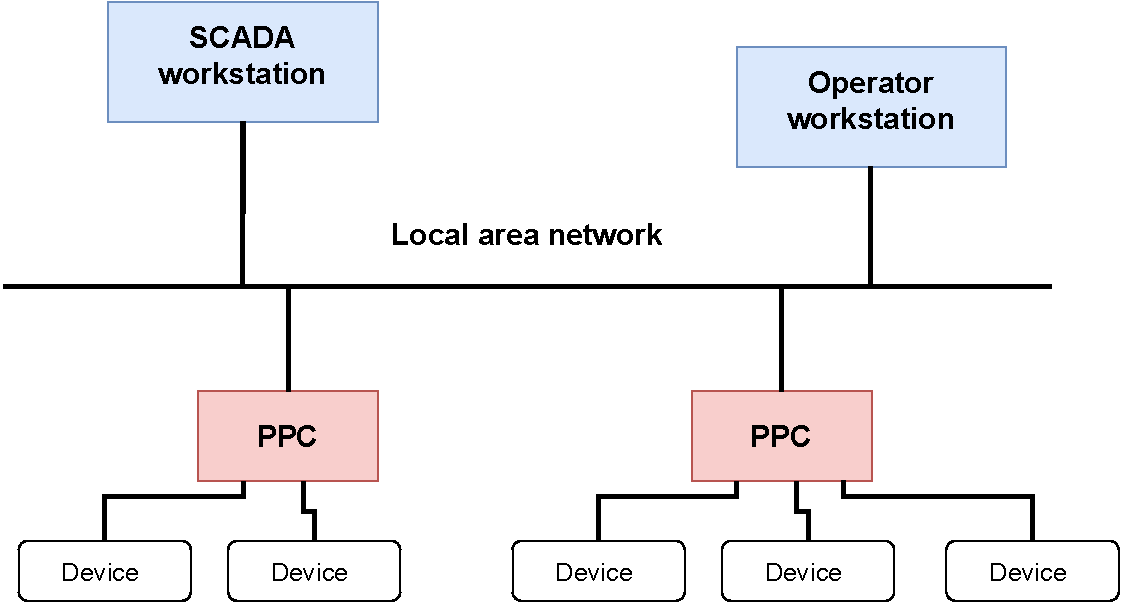
\includegraphics[scale=0.6]{images/scada_system.pdf}
    \caption{Block diagram of a typical SCADA system, based on diagram from\cite{scada_design}.}
    \label{fig: scada_system}
\end{figure}
\FloatBarrier

The image shows field devices connected to \gls{ppc}s that control them. The \gls{ppc}s are connected to the \gls{scada} \gls{hmi}, or smaller operator \gls{hmi}s through a local area network. The \gls{ppc}s are usually connected to a Local area network, where they send and retrieve data to the  \gls{hmi}s. The \gls{hmi} interfaces with the database server to process configuration and monitoring data, although some systems allow the \gls{ppc} to directly access the database.


\subsection{SCADA software development}

The life cycle of a \gls{scada}-system project is critical to understand to create a similar system. In addition, the methods involved in creating a typical \gls{scada}-system ensures the software and its documentation become well organized and structured.


\subsubsection{Input and output signals}

 First, the process areas and the field signals must be identified. The process area denotes a specific area responsible for one aspect of the operation. Each process area requires a \gls{ppc} to manage signals and a network to connect to the rest of the system.

The field signals encompass all input and output signals in a system. Knowing all signals in a system will give us an estimate of the system's requirements and aid in the development process. The input and output signals determine the configuration and monitoring processes. The input signals affect how the \gls{ppc} will control the field devices. For example, these can be discrete values that determine if a valve is open or closed or analog signals that determine voltage thresholds in a circuit. The output signals are the values monitored by the \gls{ppc}, polled by the \gls{hmi}, and stored in a database. These are usually measurements from a sensor, such as a temperature, voltage, or flow.


\subsubsection{Defining PPC operations}

The functionality of the \gls{ppc} should be defined and documented so the reader can understand how the monitor and control operations are performed. In addition, the documentation of the \gls{ppc} aids in developing the workstation software, which must interface with it.

\subsubsection{Developing workstation software}

The software to be used in the workstations comprises two parts: the system's graphical display, which serves as the \gls{hmi}, and the databases containing information of the \gls{ppc}s. The graphical display must be designed so the user can quickly and efficiently survey and control the system. Security must also be considered in the design; certain functions that can change parameter values should ideally be only available to administrative users. This reduces the chance of equipment or instruments being damaged, or data being deleted by inexperienced users.

The database software must store configuration values for the \gls{ppc}s and the monitoring data from them. There are usually two databases maintained for this purpose, one for configuration and one for monitoring. Communication software must be developed that regularly polls data from the \gls{ppc} and inserts it into the monitoring database. Likewise, the configuration software must retrieve data from the configuration database and send the data to the \gls{ppc}. The tag values used in the database should be meaningful and standardized, making it easy for users to get an overview of the data.



\subsubsection{Software documentation}
Another essential aspect of such a control system is having a consistent programming standard and a complete software documentation. \gls{scada} and similar systems often have a long shelf time, and a well-documented system will make maintenance and work in the future more manageable. In general, starting with good software documentation and expanding upon it during the project development will lead to sufficient documentation of the entire system.

Good documentation of a \gls{scada}-system includes:

\begin{itemize}
    \item Description of database architecture, along with an explanation of the tag values.
    \item Description of the PPC logic, including functions and signals involved.
    \item An operational manual for the displays and functions available to the user.
    \item A reference of the displays, programs, and databases used in the application.
\end{itemize}


\subsection{Software design}

Software design can be a complex task when developing an extensive system. Therefore, specific measures should be taken to ensure that software development and maintenance are manageable. Using programming standards and conventions can drastically increase the readability and the ease of expanding the software. Additionally, using version control systems like Git and GitHub makes maintaining the code in a project with multiple people straightforward.

\subsubsection{Object Oriented Programming}

A consistent programming standard helps debug and expand the system's functionality. For example, \gls{oop} is a prevalent programming paradigm used to structure programs and increase the code's reusability and maintainability.

\gls{oop} have four basic principles when creating classes in programs: Abstraction, Encapsulation, Inheritance, and Polymorphism. Abstraction is based on creating an object or class interface that allows an outside source to interact with the object without knowing the inner implementation of the class. This reduces the program complexity and serves as an intuitive segmenting of the software.

Encapsulation declares that only the class should be able to manipulate and interact with its private variables. This assures that the classes are not dependent on other class implementations, which increases the modularity of the software. Finally, Inheritance and Polymorphism are closely related; they describe how classes can be derived from other classes, "inheriting" their functions, and how the inherited functions can be redefined, altering the class's behaviour.


These principles guide the developer to create modular and structured software which is reusable, easy to maintain, and modify. Abstraction is the most important principle, and encapsulation relates to how to create a good abstraction of the system. These two principles will be used the most in the work of this thesis. Systems designed to manage large amounts of data acquisition, such as a \gls{pet}-scan system, have in the past used \gls{oop} to design and manage large programs\cite{pet_control_system}. This gives more credence to use \gls{oop} in similar projects.

\subsubsection{Git and GitHub}
The use of the Git and GitHub tools is essential today to manage the project code and maintain it as a version control system. The version control system is essential for verifying the code; no matter what happens, a stable version of the software will always be available in previous versions on Git or GitHub. GitHub also enables a better workflow with co-developers or mentors, allowing easy access to the source code and giving feedback. 

The GitHub repository used for this thesis contains a README file containing all practical information about the repository and the project's goals. This includes information about the configuration and monitoring process and a user guide to start the databases and \gls{gui}s. An example of the README file is given in \autoref{fig: readme}.


\begin{figure}[!ht]
    \centering
    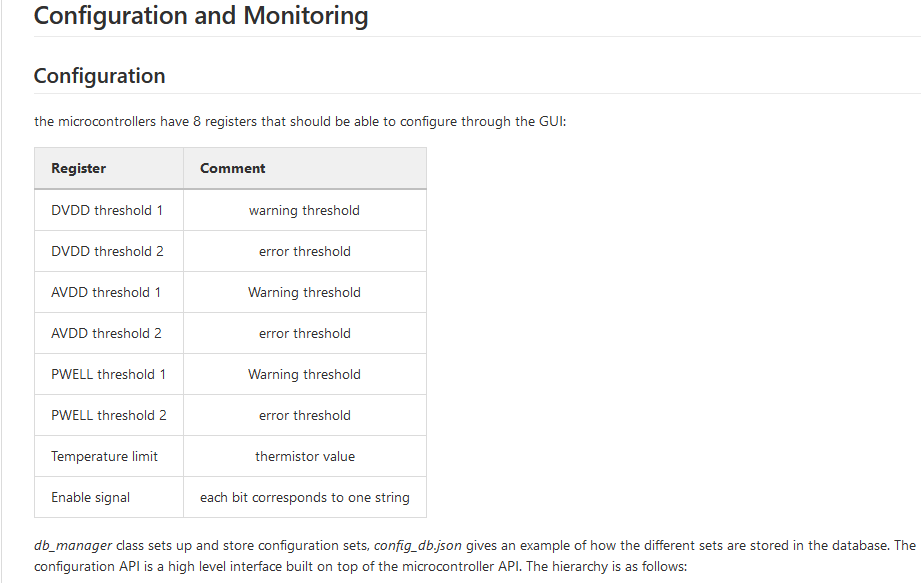
\includegraphics[width=14cm]{images/README_example.png}
    \caption{Example from the README file showing the overview of the configuration process.}
    \label{fig: readme}
\end{figure}
\FloatBarrier

\end{document}

\end{document}